\section{Contiki-ng}
\label{sec:contikiNG}

Contiki es un sistema operativo enfocado a sensores de baja capacidad. Este sistema operativo fue desarrollado por Adam Dunkels con la ayuda de  Bjorn Gronvall y Thiemo Voigt en el año 2002. Desde entonces hasta los últimos años, el proyecto Contiki  ha involucrado tanto a empresas como a cientos de colaboradores en su repositorio de GitHub\footnote{\url{https://github.com/contiki-os/contiki}}.  Contiki estaba diseñado con el propósito de ofrecer a los nodos de las redes \gls{wsn} un sistema operativo ligero con capacidad de carga y descarga de servicios únicos de forma dinámica \cite{1367266}. \\
\par
El Kernel de Contiki está orientado a eventos, y soporta tareas multi-hilo con requisa. Contiki está escrito en el lenguaje C y ha sido portado a numerosas de arquitecturas de microcontroladores, como el MSP430 de Texas Instruments y derivados. \\
\par

En un sistema que ejecute el sistema operativo de Contiki, éste estará dividido en dos partes claramente diferenciadas según se puede ver en la figura \ref{fig:contikiParts}, el \textit{core} y los programas o servicios cargados. El particionado se lleva a cabo en el momento de la compilación y es independiente de cada target en el que se vaya a desplegar el sistema. El \textit{core} consiste en el propio Kernel, un conjunto de servicios de base (\textit{timers}, \textit{handlers}) , librerías, drivers y el \textit{stack} de comunicación. Los programas o servicios cargados se mapearán en memoria por el propio cargador que tiene el Kernel en tiempo de ejecución.\\
\par


% Foto 
\begin{figure}[ht]
    \centering
    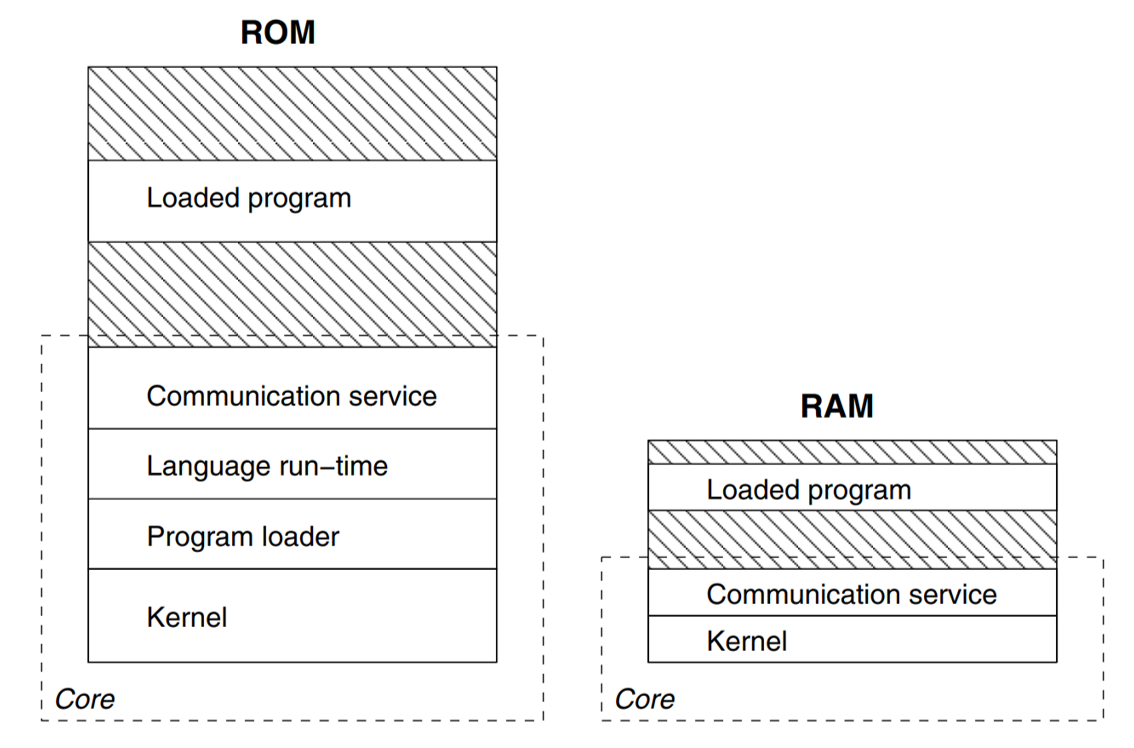
\includegraphics[width=9.5cm]{archivos/img/teoria/contiki.png}
    \caption{Particionado en un sistema con Contiki OS \cite{1367266}}
    \label{fig:contikiParts}
\end{figure}

En los últimos años apareció un nuevo proyecto, \textbf{Contiki-ng} \footnote{\url{https://github.com/contiki-ng/contiki-ng}}, el cual es fork de Contiki OS. Este nuevo proyecto desbancaría a su predecesor bajo el eslogan de ``\textit{Contiki-NG: The OS for Next Generation IoT Devices}". Actualmente toda la comunidad de Contiki está enfocada en este nuevo proyecto, el cual proporciona un \textit{stack} de comunicación más cercano a las RFCs, soporte a protocolos como IPv6/6LoWPAN y 6TiSCH, y por lo que se está haciendo más popular, dar soporte a microcontroladores con la arquitectura ARM \cite{kurniawan2018practical}.
\vspace{0.5cm}


\subsection{Simulador Cooja}

El flujo de trabajo con Contiki o Contiki-ng varía dependiendo de si se trabaja con hardware real o si se realiza una simulación de los programas desarrollados. En el caso de trabajar con hardware real, el proceso consiste en compilar el sistema operativo y los programas específicos utilizando el objetivo (target) correspondiente, lo que generará un archivo binario que se puede cargar en la memoria del hardware.\\
\\
Por otro lado, si se opta por la simulación, se utilizará el simulador llamado Cooja\footnote{\url{https://github.com/contiki-ng/cooja/tree/master}}. Cooja es un simulador escrito en Java que permite \textbf{simular} una serie de nodos \gls{iot}. Al simular, es posible observar el comportamiento del programa desarrollado en diferentes plataformas. El proceso de compilación del núcleo (core) de Contiki y los programas desarrollados está integrado en el propio simulador, lo que facilita al usuario la compilación de sus programas para diferentes tipos de nodos. Cada simulación se puede guardar en un archivo con extensión \texttt{*.csc}, que almacena todos los datos de la simulación, como la semilla (\textit{seed}), las posiciones y los tipos de nodos, utilizando una estructura XML.\\
\\
De esta manera, tanto si se trabaja con hardware real como si se realiza una simulación, Contiki y Contiki-ng ofrecen herramientas y entornos integrados que permiten desarrollar y probar programas para sistemas embebidos y dispositivos \gls{iot}. A continuación, en la figura \ref{fig:cooja}, se indica la interfaz gráfica del simulador.

\begin{figure}[ht]
    \centering
    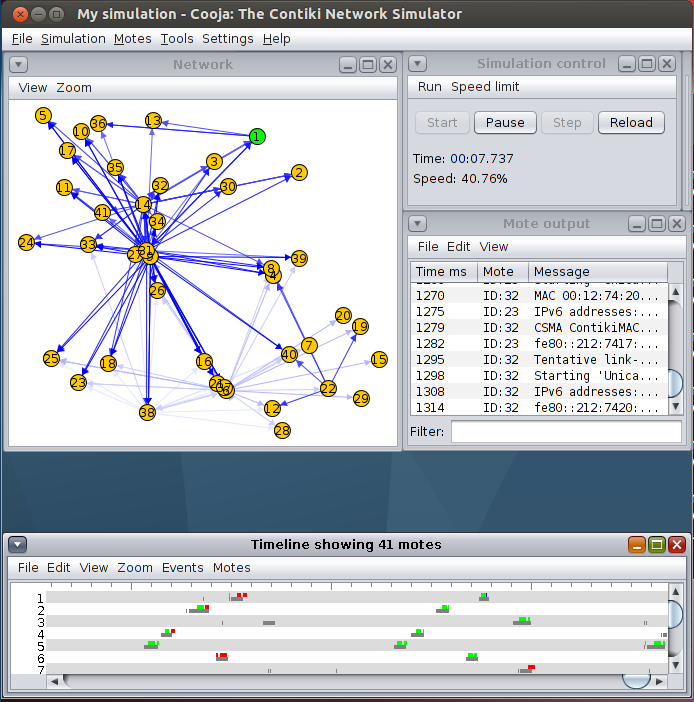
\includegraphics[width=0.6\textwidth]{archivos/img/teoria/cooja.png}
    \caption{Interfaz gráfica del simulador Cooja \cite{cooja1}}
    \label{fig:cooja}
\end{figure}

